\documentclass[11pt]{article}

\usepackage[utf8]{inputenc}
\usepackage[T1]{fontenc}
\usepackage[spanish,es-noshorthands]{babel}
\usepackage{listings}
\usepackage{graphicx}
\usepackage{float}
\usepackage{hyperref}
\usepackage{booktabs}
\usepackage{xcolor}
\usepackage{geometry}
\geometry{margin=2.5cm}

\hypersetup{colorlinks=true, linkcolor=blue!50!black, urlcolor=blue!50!black,
            citecolor=blue!50!black}

% ----------------- Estilo de listados (código y salidas) -----------------
\definecolor{codebg}{RGB}{248,248,248}
\definecolor{codekw}{RGB}{37,99,235}
\definecolor{codecomment}{RGB}{22,128,80}
\definecolor{codestr}{RGB}{180,60,30}

\lstset{
  basicstyle=\ttfamily\footnotesize,
  backgroundcolor=\color{codebg},
  frame=single,
  framerule=0.3pt,
  rulecolor=\color{gray!40},
  breaklines=true,
  postbreak=\mbox{\textcolor{gray}{$\hookrightarrow$}\space},
  columns=fullflexible,
  keepspaces=true,
  showstringspaces=false,
  inputencoding=utf8,
  extendedchars=true,
  literate=%
    {á}{{\'a}}1 {é}{{\'e}}1 {í}{{\'i}}1 {ó}{{\'o}}1 {ú}{{\'u}}1
    {Á}{{\'A}}1 {É}{{\'E}}1 {Í}{{\'I}}1 {Ó}{{\'O}}1 {Ú}{{\'U}}1
    {ñ}{{\~n}}1 {Ñ}{{\~N}}1 {ü}{{\"u}}1 {¿}{{?`}}1 {¡}{{!`}}1
    {°}{{\textdegree}}1 {–}{{-}}1 {—}{{---}}1
}

\lstdefinestyle{python}{
  language=Python,
  keywordstyle=\color{codekw}\bfseries,
  commentstyle=\color{codecomment}\itshape,
  stringstyle=\color{codestr},
}
\lstdefinestyle{salida}{
  basicstyle=\ttfamily\scriptsize,
  keywordstyle=\color{black},
}

\title{}
\date{}

\begin{document}

% ============================ PORTADA ============================
\begin{titlepage}
\centering
\vspace*{1.5cm}
{\Large\scshape Universidad Diego Portales\par}
\vspace{0.3cm}
{\large Facultad de Ingeniería y Ciencias\par}
{\large Ingeniería en Informática\par}
\vspace{2.5cm}
\rule{\linewidth}{0.5pt}\\[0.4cm]
{\huge\bfseries Tarea 3: Inyección y Modificación\\[0.2cm] de Tráfico con Scapy\par}
\vspace{0.3cm}
{\large Protocolo PostgreSQL Frontend/Backend (Wire Protocol)\par}
\rule{\linewidth}{0.5pt}\\[1.5cm]

{\large\itshape Taller de Redes y Servicios\par}
\vspace{2.0cm}

\begin{tabular}{rl}
\textbf{Estudiantes:} & Luciano Olivieri \\
                      & Alan Troncoso \\[0.3cm]
\textbf{Profesor:}    & Diego Pineda \\
\textbf{Sección:}     & 3 \\
\end{tabular}

\vfill
{\large Taller de Redes y Servicios 2026--1\par}
{\large \today\par}
\end{titlepage}

\tableofcontents
\newpage

% ============================ 1. INTRODUCCIÓN ============================
\section{Introducción}

Esta tarea continúa el trabajo de la Tarea~2, donde se instaló y analizó la
dupla cliente/servidor de \textbf{PostgreSQL} (\texttt{psql} y \texttt{postgres})
y se caracterizó el protocolo de aplicación que ambos hablan: el
\emph{Frontend/Backend Protocol v3.0}~\cite{pgprotocol}. Mientras que en la
Tarea~2 el tráfico se observó de forma pasiva con \texttt{tcpdump} y Wireshark,
aquí se adopta un rol \textbf{activo}: se intercepta el tráfico en tiempo real,
se inyectan y modifican mensajes del protocolo, y se mide cómo reacciona el
servicio ante entradas no esperadas y ante la degradación de métricas de red.

\subsection{Descripción del servicio}
PostgreSQL es un sistema gestor de bases de datos relacional cliente--servidor.
El cliente envía órdenes SQL y el servidor las ejecuta y responde. La
comunicación viaja sobre TCP (puerto 5432) mediante un protocolo orientado a
mensajes: salvo el \emph{StartupMessage} y el \emph{SSLRequest} iniciales, cada
mensaje comienza con un byte ASCII de tipo, seguido de un entero de 4 bytes con
la longitud total y luego el contenido~\cite{pgmessageformats}. Tal como se
documentó en la Tarea~2, cuando no se habilita TLS todo el intercambio
posterior a la autenticación viaja en texto plano: las consultas SQL y los datos
devueltos son legibles en el cable. La contraseña es la única excepción, gracias
al mecanismo SCRAM-SHA-256~\cite{rfc5802}.

\subsection{Arquitectura del entorno}
El escenario se compone de tres contenedores Docker sobre una red \emph{bridge}
dedicada (\texttt{redpsql}, subred \texttt{172.18.0.0/16}):

\begin{itemize}
  \item \textbf{servidor} (\texttt{psql-servidor}, \texttt{172.18.0.2}):
        PostgreSQL~17, idéntico al de la Tarea~2 (rol \texttt{taller}, base
        \texttt{tallerdb}, tabla \texttt{routers}, autenticación
        SCRAM-SHA-256).
  \item \textbf{cliente} (\texttt{psql-cliente}, \texttt{172.18.0.3}): aporta el
        binario \texttt{psql}; desde él se generan las sesiones.
  \item \textbf{scapy} (\texttt{scapy\_mitm}, \texttt{172.18.0.4}): contenedor
        nuevo de la Tarea~3, con Scapy, \texttt{tcpdump}, \texttt{iproute2}
        (\texttt{tc}) y los scripts de inyección/modificación. Corre como
        \texttt{privileged} con \texttt{NET\_ADMIN} y \texttt{NET\_RAW}.
\end{itemize}

\subsection{Herramientas utilizadas}
Scapy~\cite{scapy} y \texttt{sockets} de Python para construir e interceptar
mensajes; un \textbf{proxy TCP MITM} propio para la modificación al vuelo;
\texttt{tc qdisc netem}~\cite{netem} para inyectar latencia y pérdida de
paquetes; \texttt{matplotlib} para graficar; y Docker para orquestar el
entorno~\cite{dockernet}.

\paragraph{Nota de reproducibilidad.} Todos los experimentos de este informe
---\emph{fuzzing}, \emph{modificaciones} y \emph{métricas}--- se ejecutaron en el
entorno Docker real descrito arriba: los tres contenedores sobre la red
\texttt{redpsql}, con PostgreSQL~17 (mismo rol, base, tabla y autenticación
SCRAM-SHA-256 que la Tarea~2). Las salidas mostradas son la captura literal de
cada ejecución y se incluyen completas en el directorio \texttt{capturas/}. Las
dos métricas (latencia y pérdida) se midieron con \texttt{tc qdisc netem} real
aplicado sobre la interfaz \texttt{eth0} del contenedor cliente, mediante los
scripts \texttt{metric1\_latency.sh} y \texttt{metric2\_loss.sh}.

% ===================== 2. PROTOCOLO ==========================
\section{Descripción del Protocolo PostgreSQL Wire Protocol}

\subsection{Estructura de mensajes}
Un mensaje regular del protocolo v3.0 tiene la forma:
\begin{center}
\texttt{[ tipo : 1 byte ] [ length : 4 bytes (big-endian) ] [ payload : length-4 bytes ]}
\end{center}
El campo \texttt{length} incluye sus propios 4 bytes pero no el byte de tipo.
Gracias a este encabezado fijo, el receptor sabe siempre dónde termina un
mensaje, incluso si varios llegan juntos en un mismo segmento TCP. Los dos
primeros mensajes del cliente son especiales: el \emph{SSLRequest} y el
\emph{StartupMessage} \textbf{no} llevan byte de tipo (por compatibilidad
histórica) y comienzan directamente con el campo \texttt{length}.

\subsection{Tipos de mensaje utilizados}
\begin{table}[H]
\centering
\caption{Mensajes del protocolo frontend/backend relevantes para esta tarea.}
\begin{tabular}{cll}
\toprule
\textbf{Byte} & \textbf{Mensaje} & \textbf{Emisor / Propósito} \\
\midrule
-- & StartupMessage   & Cliente: abre la sesión (usuario, base, parámetros) \\
\texttt{Q} (0x51) & Query            & Cliente: texto SQL (consulta simple) \\
\texttt{X} (0x58) & Terminate        & Cliente: cierre ordenado de la sesión \\
\texttt{p} (0x70) & PasswordMessage  & Cliente: respuesta SASL/SCRAM \\
\texttt{R} (0x52) & Authentication   & Servidor: solicita/confirma autenticación \\
\texttt{T} (0x54) & RowDescription   & Servidor: describe columnas del resultado \\
\texttt{D} (0x44) & DataRow          & Servidor: una fila del resultado \\
\texttt{C} (0x43) & CommandComplete  & Servidor: resumen de la orden \\
\texttt{Z} (0x5A) & ReadyForQuery    & Servidor: listo para recibir órdenes \\
\texttt{E} (0x45) & ErrorResponse    & Servidor: informe de error \\
\texttt{S} (0x53) & ParameterStatus  & Servidor: parámetro de configuración \\
\texttt{K} (0x4B) & BackendKeyData   & Servidor: PID y clave de cancelación \\
\bottomrule
\end{tabular}
\end{table}

\subsection{Estructura del StartupMessage}
\begin{center}
\texttt{[ length : 4 ] [ protocol : 4 ] [ clave\textbackslash0valor\textbackslash0 ... \textbackslash0 ]}
\end{center}
El campo \texttt{protocol} se codifica como \texttt{(major<<16) | minor}; para la
versión 3.0 vale \texttt{196608} (\texttt{0x00030000}). A continuación van pares
clave/valor terminados en \texttt{\textbackslash0} (típicamente \texttt{user} y
\texttt{database}) y un \texttt{\textbackslash0} final que cierra el bloque. La
mayoría de los casos de \emph{fuzzing} de la Sección~\ref{sec:fuzz2} atacan
precisamente estos campos.

% ===================== 3. INTERCEPTACIÓN ==========================
\section{Interceptación con Scapy}

La interceptación se aborda con dos herramientas complementarias. Para la
\textbf{observación pasiva} se usa \textbf{Scapy}: el script
\texttt{sniffer\_scapy.py} ejecuta \texttt{sniff()} sobre la interfaz de la red
\texttt{redpsql} (filtro \texttt{tcp port 5432}) y diseca cada segmento,
identificando los tipos de mensaje del protocolo (\texttt{Q}, \texttt{T},
\texttt{D}, \texttt{C}, \texttt{Z}, \texttt{E}, \texttt{p}, \texttt{R}, \dots).
Para la \textbf{modificación activa} se usa un proxy TCP MITM. Esta división es
deliberada: reescribir un flujo TCP \emph{con estado} exige terminar la conexión
TCP en el intermediario, algo que la inyección de paquetes sueltos de Scapy no
realiza de forma fiable; Scapy es óptimo para capturar y diseccionar, y el proxy
para reescribir el \emph{stream}.

\subsection{Arquitectura del proxy MITM}
La modificación en tiempo real se realiza con un \textbf{proxy TCP transparente}
(\emph{man-in-the-middle}) que se interpone entre el cliente y el servidor:

\begin{center}
\begin{minipage}{0.92\linewidth}
\begin{verbatim}
   cliente (psql)            scapy_mitm (proxy :5433)            servidor (:5432)
        |  --- Q "SELECT 1" --->  |                                   |
        |                         |  [ client_to_server_hook ]        |
        |                         |  --- Q' (modificado) ----------->  |
        |                         |                                   |
        |                         |  <---- T / D / C / Z / E --------  |
        |  <--- respuesta ------  |  [ server_to_client_hook ]        |
\end{verbatim}
\end{minipage}
\end{center}

El proxy escucha en el puerto \texttt{5433}, abre una conexión al servidor real
(\texttt{5432}) por cada cliente y reenvía los bytes en \textbf{dos hilos}
independientes (uno por sentido). Cada sentido aplica un \emph{hook} opcional que
puede inspeccionar y reescribir el payload antes de retransmitirlo. Este diseño
permite implementar todas las modificaciones de la Sección~\ref{sec:mods} sin
tocar ni el cliente ni el servidor: para ellos, el proxy es indistinguible del
otro extremo. Esto es posible precisamente porque el canal no está cifrado;
con \texttt{sslmode=require} el \emph{handshake} TLS detectaría al intermediario.

\subsection{Código del proxy base}
\begin{lstlisting}[style=python, caption={Núcleo del proxy MITM (\texttt{mitm\_proxy.py}).}]
class PgMITMProxy:
    def handle_client(self, client_sock, addr):
        # Por cada cliente abre la conexión al servidor real y lanza dos relays
        server_sock = socket.socket(socket.AF_INET, socket.SOCK_STREAM)
        server_sock.connect((self.server_host, self.server_port))
        t1 = threading.Thread(target=self._relay,
                 args=(client_sock, server_sock, self.c2s_hook, "C->S"))
        t2 = threading.Thread(target=self._relay,
                 args=(server_sock, client_sock, self.s2c_hook, "S->C"))
        t1.start(); t2.start(); t1.join(); t2.join()

    def _relay(self, src, dst, hook, direction):
        while not self._stop.is_set():
            data = src.recv(BUFSIZE)
            if not data:
                break                      # cierre ordenado
            out = hook(data) if hook else data   # aplica la modificación
            dst.sendall(out)
\end{lstlisting}

% ===================== 4. FUZZING ==========================
\section{Experimentos de Fuzzing}

Se implementaron dos inyecciones con \textbf{técnicas de fuzzing distintas}: una
de generación pura (datos aleatorios) y otra de mutación dirigida sobre un
mensaje válido. En ambos casos el objetivo es comprobar la robustez del
\emph{parser} del servidor ante entradas no esperadas.

\subsection{Fuzzing 1: payload aleatorio}
\label{sec:fuzz1}
\textbf{Técnica: \emph{dumb fuzzing} / generación.} Se generan 10 paquetes de
bytes completamente aleatorios (tamaño 10--1000~B, semilla fija para
reproducibilidad) y se envían directamente al servidor, sin ninguna estructura
del protocolo. Tras cada envío se clasifica la respuesta y se verifica que el
servidor siga vivo enviando un \emph{SSLRequest} de sondeo.

\begin{lstlisting}[style=python, caption={Bucle principal de \texttt{fuzzing\_1.py}.}]
for i in range(1, N_ITER + 1):
    size = random.randint(MIN_SIZE, MAX_SIZE)
    payload = bytes(random.randint(0, 255) for _ in range(size))
    s = socket.create_connection((SERVER_HOST, SERVER_PORT), timeout=TIMEOUT)
    s.sendall(payload)
    resp = s.recv(4096)                  # respuesta del servidor
    estado = classify(resp, ...)         # 'E', timeout, cierre, ...
    alive, _ = server_alive(SERVER_HOST, SERVER_PORT)
\end{lstlisting}

\textbf{Comportamiento esperado.} PostgreSQL interpreta los primeros 4 bytes como
el \texttt{length} del StartupMessage. Con bytes aleatorios, ese length casi
siempre resulta inválido (negativo o mayor que el máximo de
\texttt{10000}~bytes que admite un \emph{startup packet}), por lo que el servidor
debe rechazar la conexión sin procesarla y sin caerse.

\textbf{Resultado observado (real).}
\begin{lstlisting}[style=salida]
[Iteración  1] tamaño=642 bytes  (21.6 ms)
   primeros 16 bytes enviados : 22 96 a3 ... (aleatorios)
   CLASIFICACIÓN              : el servidor cerró la conexión sin responder
   ¿Servidor sigue vivo?      : SÍ -> vivo (respondió 'N' al SSLRequest)
...
   El servidor PostgreSQL SOBREVIVIÓ tras las 10 iteraciones de fuzzing.
\end{lstlisting}

\textbf{Análisis.} En las 10 iteraciones el servidor cerró la conexión sin
emitir datos y permaneció operativo. El \emph{length} aleatorio supera de forma
sistemática el máximo permitido para un \emph{startup packet}, de modo que el
\emph{postmaster} aborta la conexión (registra \texttt{invalid length of startup
packet}) antes de leer el resto. El \emph{dumb fuzzing} confirma la robustez del
primer punto de entrada, pero ejercita rutas de parsing muy superficiales:
prácticamente todos los casos mueren en la misma validación. Esto motiva el
segundo experimento.

\subsection{Fuzzing 2: StartupMessage mutado}
\label{sec:fuzz2}
\textbf{Técnica: \emph{mutation-based fuzzing} + \emph{bit-flipping}.} Se parte
de un StartupMessage \textbf{válido} y se le aplican mutaciones dirigidas a
campos concretos. Al ser semillas válidas ligeramente corrompidas, el servidor
las acepta lo suficiente como para alcanzar rutas de parsing más profundas que
en el Fuzzing~1.

\begin{lstlisting}[style=python, caption={Constructor del mensaje semilla y bit-flip (\texttt{fuzzing\_2.py}).}]
def build_startup(user, db, major=3, minor=0):
    protocol = (major << 16) | minor                  # 196608 para v3.0
    params = ("user\x00%s\x00database\x00%s\x00"
              "application_name\x00psql\x00" % (user, db)).encode() + b"\x00"
    length = 4 + 4 + len(params)
    return struct.pack(">II", length, protocol) + params

def bitflip(data, n):                                 # n bit-flips aleatorios
    b = bytearray(data)
    for _ in range(n):
        b[random.randint(0, len(b)-1)] ^= (1 << random.randint(0, 7))
    return bytes(b)
\end{lstlisting}

\begin{table}[H]
\centering
\caption{Casos de Fuzzing 2 y respuesta real del servidor PostgreSQL 17.}
\label{tab:fuzz2}
\begin{tabular}{cp{6.4cm}p{6.0cm}}
\toprule
\textbf{\#} & \textbf{Mutación aplicada} & \textbf{Respuesta del servidor} \\
\midrule
1 & Protocol version 99.0 (\texttt{0x00630000}) & \texttt{FATAL 0A000: unsupported frontend protocol 99.0: server supports 3.0 to 3.0} \\
2 & \texttt{length = 0xFFFFFFFF} (\(\sim\)4 GB)  & El servidor cierra la conexión (\emph{invalid message length}) \\
3 & \texttt{length = 0}                          & El servidor cierra la conexión \\
4 & Username con null embebido \texttt{post\textbackslash0gres} & \texttt{FATAL 08P01: invalid startup packet layout: expected terminator as last byte} \\
5 & Bit-flip en 5 posiciones aleatorias          & \texttt{FATAL 08P01: invalid startup packet layout...} \\
6 & Startup sin terminador final \texttt{\textbackslash0} & \texttt{FATAL 08P01: invalid startup packet layout...} \\
7 & Sólo 4 bytes (\texttt{length=8}, sin protocolo) & \textbf{Timeout}: el servidor queda esperando más bytes \\
8 & Username de 10.000 caracteres                & El servidor cierra la conexión (excede el máximo del \emph{startup packet}) \\
\bottomrule
\end{tabular}
\end{table}

\textbf{Análisis.} A diferencia del Fuzzing~1, aquí cada caso provoca una
reacción \emph{distinta}, lo que demuestra que el servidor valida por capas:
primero el tamaño del paquete (casos 2, 3, 8), luego la versión de protocolo
(caso 1) y finalmente la estructura de los pares clave/valor (casos 4, 5, 6,
que comparten el error \texttt{08P01}). El caso~7 es especialmente
ilustrativo: un \texttt{length} válido pero sin el resto del mensaje deja al
backend \emph{bloqueado} esperando bytes que no llegan ---un anticipo del
comportamiento de la Modificación~2 (Sección~\ref{sec:mod2}). En los 8 casos el
\emph{postmaster} siguió operativo: ninguno logró tumbar el servidor.

% ===================== 5. MODIFICACIONES ==========================
\section{Modificaciones de Protocolo}
\label{sec:mods}

Las tres modificaciones usan el proxy MITM de la Sección~3. Para obtener salidas
limpias y deterministas, un cliente interno (que implementa el protocolo y la
autenticación SCRAM) envía una consulta concreta a través del proxy, y el
\emph{hook} la altera al vuelo.

\subsection{Modificación 1: byte de tipo de mensaje}
\label{sec:mod1}
\textbf{Fundamentación.} El byte de tipo le dice al servidor cómo interpretar el
mensaje. Si se reescribe, el receptor pierde la sincronía del flujo. Se esperan
tres comportamientos: (A) \texttt{Q}$\to$\texttt{X} debe interpretarse como
\emph{Terminate} y cerrar la sesión limpiamente; (B) \texttt{Q}$\to$\texttt{0xFF}
es un tipo inexistente y debe gatillar un error fatal de protocolo; (C)
\texttt{Q}$\to$\texttt{p} entrega un \emph{PasswordMessage} fuera de la fase de
autenticación, que el bucle de comandos tampoco reconoce.

\begin{lstlisting}[style=python, caption={Hook que reescribe el byte de tipo (\texttt{mod\_1\_message\_type.py}).}]
def make_hook(new_type):
    def hook(data):
        if data[:1] == b"Q":                       # detecta el Query
            return bytes([new_type]) + data[1:]    # cambia sólo el byte de tipo
        return data
    return hook
\end{lstlisting}

\textbf{Resultado observado (real).}
\begin{lstlisting}[style=salida]
 CASO A: 'Q' (0x51) -> 'X' (0x58, Terminate)
   Respuesta del servidor (0.0 ms):
       Conexión cerrada por el servidor
 CASO B: 'Q' (0x51) -> 0xFF (tipo inexistente)
   Respuesta del servidor (0.0 ms):
       ErrorResponse -> FATAL 08P01: invalid frontend message type 255
 CASO C: 'Q' (0x51) -> 'p' (0x70, PasswordMessage)
   Respuesta del servidor (0.0 ms):
       ErrorResponse -> FATAL 08P01: invalid frontend message type 112
\end{lstlisting}

\textbf{Comportamiento observado vs.\ esperado.} Los tres casos coincidieron con
lo esperado. En (A) el servidor trató el mensaje como \emph{Terminate} y cerró la
conexión sin enviar resultados; el cliente no recibe ninguna respuesta a su
``\texttt{SELECT 1}''. En (B) y (C) el servidor emitió un \texttt{ErrorResponse}
\textbf{FATAL} con código \texttt{08P01} (\emph{protocol violation}):
\texttt{invalid frontend message type 255} y \texttt{112} respectivamente
(\texttt{0xFF} y \texttt{0x70} en decimal), y cerró la conexión. Esto valida la
hipótesis~3 de la Tarea~2: corromper el encabezado produce un error estructural,
no un resultado adulterado.

\subsection{Modificación 2: campo length}
\label{sec:mod2}
\textbf{Fundamentación.} El \texttt{length} indica cuántos bytes leer del stream.
Con \texttt{length} mayor al real (A), el servidor quedará esperando bytes que
nunca llegan y la sesión se bloqueará hasta un timeout; con \texttt{length}
demasiado corto (B), el servidor leerá una cadena truncada; con un
\texttt{length} absurdo (C), debe activarse la validación de longitud máxima.

\begin{lstlisting}[style=python, caption={Hook que altera el campo length (\texttt{mod\_2\_length.py}).}]
def make_hook(mode, delta):
    def hook(data):
        if data[:1] == b"Q" and len(data) >= 5:
            real = struct.unpack(">I", data[1:5])[0]
            new = {"add": real+delta, "sub": real-delta, "max": 0xFFFFFFFF}[mode]
            return data[:1] + struct.pack(">I", new & 0xFFFFFFFF) + data[5:]
        return data
    return hook
\end{lstlisting}

\textbf{Resultado observado (real).}
\begin{lstlisting}[style=salida]
 CASO A: length_real + 1000  ->  length real=13 -> falso=1013
   Tiempo de respuesta: 4000.1 ms
       RESULTADO: TIMEOUT -> el backend quedó BLOQUEADO esperando bytes extra.
       ¿Servidor sigue vivo? SÍ
 CASO B: length_real - 4  ->  length real=13 -> falso=9
       ErrorResponse -> ERROR 08P01: invalid string in message
 CASO C: 0xFFFFFFFF  ->  length real=13 -> falso=4294967295
       Conexión cerrada por el servidor (invalid message length)
\end{lstlisting}

\textbf{Comportamiento observado vs.\ esperado.} Coincidió en lo esencial. El
caso~(A) confirma el bloqueo previsto: tras inyectar \texttt{length+1000} el
backend esperó 1000 bytes adicionales y el cliente tuvo que abortar por
\emph{timeout} a los 4~s; la sesión quedó colgada, pero el servidor siguió
atendiendo nuevas conexiones (cada sesión es un proceso \emph{forked}
independiente). El caso~(B) produjo \texttt{invalid string in message}: al leer
sólo 5 de los 9 bytes del cuerpo, el texto SQL quedó sin su terminador nulo y el
\emph{parser} lo rechazó. El caso~(C) gatilló la validación de longitud máxima y
el servidor cerró la conexión. En ningún caso cayó el \emph{postmaster}.

\subsection{Modificación 3: contenido de la query SQL}
\label{sec:mod3}
\textbf{Fundamentación.} Como el protocolo sin TLS no integra verificación de
integridad, un MITM puede reescribir el texto SQL sin que ninguno de los dos
extremos lo note. Se esperan tres efectos: (A) inyectar \texttt{pg\_sleep(5)}
añade 5~s de latencia visible; (B) redirigir la tabla produce un error
\texttt{42P01}; (C) añadir \texttt{WHERE 1=0} vacía el resultado sin error.

\begin{lstlisting}[style=python, caption={Hook que reescribe el SQL y reconstruye el mensaje (\texttt{mod\_3\_query.py}).}]
def make_hook(mode):
    def hook(data):
        if data[:1] == b"Q" and len(data) >= 5:
            length = struct.unpack(">I", data[1:5])[0]
            sql = data[5:1+length].split(b"\x00")[0].decode()
            sql2 = rewrite_sql(sql, mode)            # pg_sleep / tabla / WHERE 1=0
            body = sql2.encode() + b"\x00"
            return b"Q" + struct.pack(">I", 4+len(body)) + body
        return data
    return hook
\end{lstlisting}

\textbf{Resultado observado (real).}
\begin{lstlisting}[style=salida]
 CASO A: SELECT -> SELECT pg_sleep(5)
   [hook] SQL original  del cliente : 'SELECT 1'
   [hook] SQL modificado al servidor: 'SELECT pg_sleep(5)'
   Respuesta observada por el cliente (5006 ms)  ->  esperó ~5.0 s
 CASO B: FROM routers -> FROM tabla_inexistente_xyz
   Respuesta -> ERROR 42P01: relation "tabla_inexistente_xyz" does not exist
 CASO C: añadir WHERE 1=0  ->  'SELECT * FROM routers WHERE 1=0'
   CommandComplete: SELECT 0   (4 filas esperadas, 0 recibidas)
\end{lstlisting}

\textbf{Comportamiento observado vs.\ esperado.} Los tres casos coincidieron
exactamente. En (A) el cliente envió ``\texttt{SELECT 1}'' (respuesta
instantánea) pero esperó \textbf{5006~ms}, porque el servidor ejecutó
\texttt{pg\_sleep(5)}. En (B) el cliente consultó una tabla \emph{válida} y
recibió \texttt{42P01 relation does not exist}. En (C) el cliente esperaba 4
filas y recibió 0, sin ningún error que lo alertara. Esta modificación es la más
relevante para la seguridad: demuestra empíricamente que, sin TLS, un atacante
puede alterar la \textbf{semántica} de las consultas de forma totalmente
transparente para ambos extremos.

% ===================== 6. MÉTRICAS ==========================
\section{Métricas de Red y Cotas de Desempeño}
\label{sec:metricas}

Se eligieron dos métricas \textbf{distintas a throughput y goodput}, que miden
\textbf{aspectos diferentes} de la red: la \emph{latencia} (retardo temporal) y
la \emph{pérdida de paquetes} (fiabilidad). Por cada una se grafica cómo varía
el throughput del enlace y se identifica la \textbf{cota de desempeño}: el valor
a partir del cual el servicio se degrada de forma inaceptable.

\subsection{Métrica 1: Latencia (RTT)}
\textbf{Definición y relevancia.} La latencia es el retardo de ida y vuelta de
los paquetes. PostgreSQL es un protocolo orientado a conexión y
\emph{pregunta--respuesta}: cada consulta simple implica al menos un RTT. Por
ello, el throughput de consultas por segundo es muy sensible a la latencia, sobre
todo en cargas interactivas/OLTP que no usan \emph{pipelining}.

\textbf{Método.} Se aplicó \texttt{tc qdisc add dev eth0 root netem delay D}
sobre la interfaz del contenedor cliente (script \texttt{metric1\_latency.sh}) y,
por cada valor de delay, se midió el tiempo de 100 consultas \texttt{SELECT 1}
reales contra el servidor. Se usan 100 \emph{round-trips} separados (no un bucle
\texttt{DO} en el servidor, que incurriría en un solo RTT) para que la latencia
afecte a cada consulta.

\begin{table}[H]
\centering
\caption{Latencia vs throughput (medición real, 100 consultas por punto).}
\label{tab:lat}
\begin{tabular}{rrr l}
\toprule
\textbf{Delay (ms)} & \textbf{Throughput (ops/s)} & \textbf{Tiempo (ms)} & \textbf{Estado} \\
\midrule
0    & 216{,}7 & 461{,}5      & estable \\
10   & 64{,}8  & 1\,544{,}3   & estable \\
50   & 17{,}4  & 5\,747{,}9   & estable \\
100  & 9{,}1   & 10\,988{,}7  & estable (cota) \\
200  & 4{,}7   & 21\,475{,}4  & degradado \\
300  & 3{,}1   & 31\,989{,}0  & degradado \\
500  & 1{,}9   & 52\,970{,}2  & degradado \\
1000 & 0{,}95  & 105\,491{,}8 & degradado \\
\bottomrule
\end{tabular}
\end{table}

\begin{figure}[H]
\centering
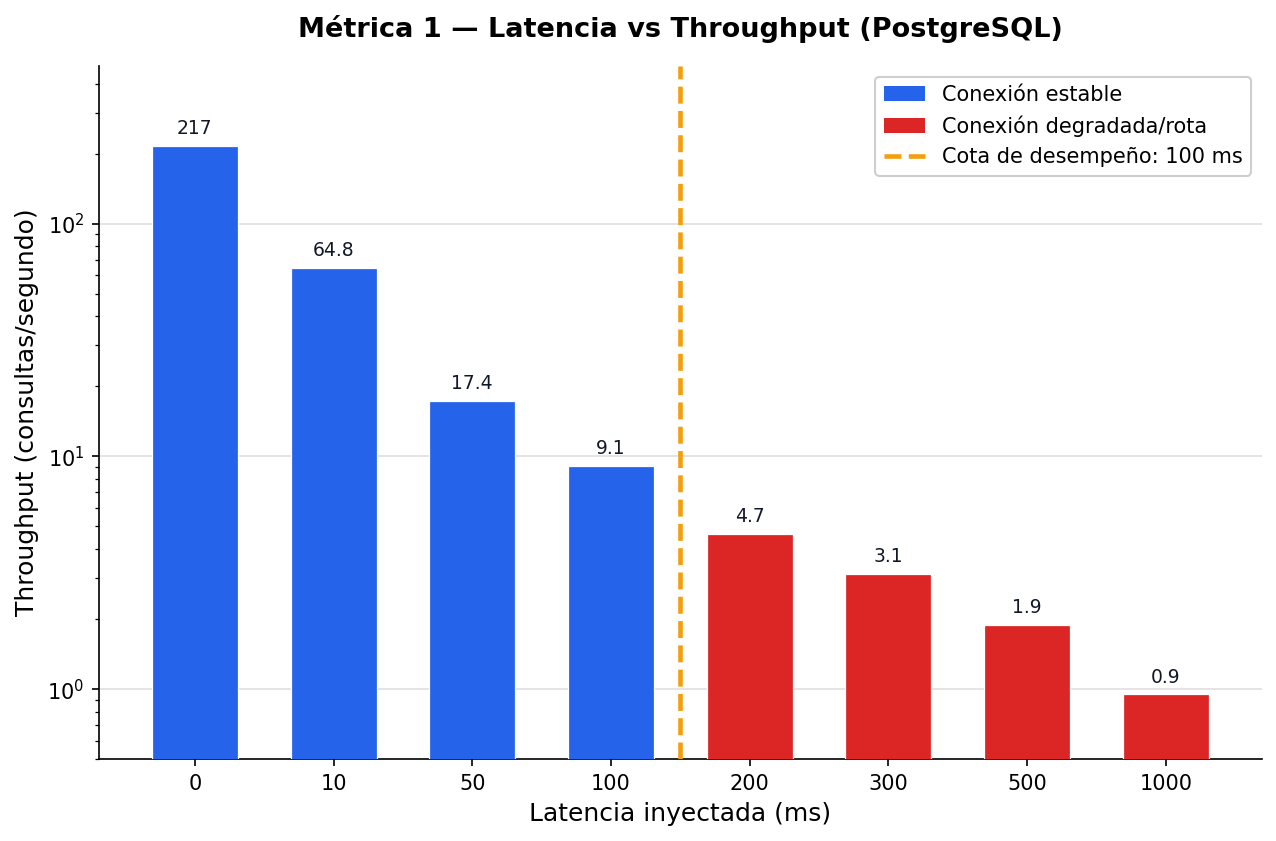
\includegraphics[width=\linewidth]{imagenes/grafico_latencia.png}
\caption{Métrica 1: latencia inyectada vs throughput. La línea punteada marca la
cota de desempeño.}
\end{figure}

\textbf{Cota de desempeño.} El throughput se mantiene en niveles operacionales
($\geq 5$~ops/s por conexión) hasta \textbf{100~ms} de latencia inyectada; a
partir de 200~ms cae por debajo de ese umbral y sigue degradándose de forma
hiperbólica hasta $\sim$1~ops/s a 1000~ms. La \textbf{cota de desempeño es
100~ms}: más allá de ese valor, el servicio interactivo/OLTP se vuelve inviable
en la práctica, aunque la conexión TCP \emph{no} llegue a romperse (TCP tolera
RTT altos). El umbral de 5~ops/s representa el mínimo razonable para una carga
transaccional sin \emph{pipelining}.

\subsection{Métrica 2: Pérdida de paquetes}
\textbf{Definición y relevancia.} La pérdida de paquetes mide la fiabilidad del
enlace. TCP la enmascara con retransmisiones, pero cada paquete perdido cuesta
un \emph{timeout} de retransmisión (RTO) muy superior al RTT, lo que degrada el
throughput de forma no lineal y, a partir de cierto umbral, hace inviable la
conexión.

\textbf{Método.} Se aplicó \texttt{tc qdisc add dev eth0 root netem loss L\%}
sobre la interfaz del contenedor cliente (script \texttt{metric2\_loss.sh}) y se
midió el throughput de 100 consultas reales por cada nivel de pérdida. La
degradación observada sigue la forma esperada para TCP: cada paquete perdido
cuesta un \emph{timeout} de retransmisión (RTO) muy superior al RTT, lo que
degrada el throughput de forma no lineal, en línea con el modelo de Mathis et
al.~\cite{mathis1997}.

\begin{table}[H]
\centering
\caption{Pérdida de paquetes vs throughput (medición real con \texttt{tc netem}).}
\label{tab:loss}
\begin{tabular}{rrr l}
\toprule
\textbf{Pérdida (\%)} & \textbf{Throughput (ops/s)} & \textbf{Tiempo (ms)} & \textbf{Estado} \\
\midrule
0  & 188{,}4 & 530{,}9      & estable \\
1  & 111{,}1 & 899{,}9      & estable \\
5  & 58{,}5  & 1\,708{,}2   & estable \\
10 & 28{,}1  & 3\,554{,}1   & estable \\
20 & 13{,}3  & 7\,539{,}3   & estable \\
30 & 8{,}3   & 11\,994{,}4  & estable (cota) \\
50 & 1{,}7   & 57\,476{,}9  & degradado \\
\bottomrule
\end{tabular}
\end{table}

\begin{figure}[H]
\centering
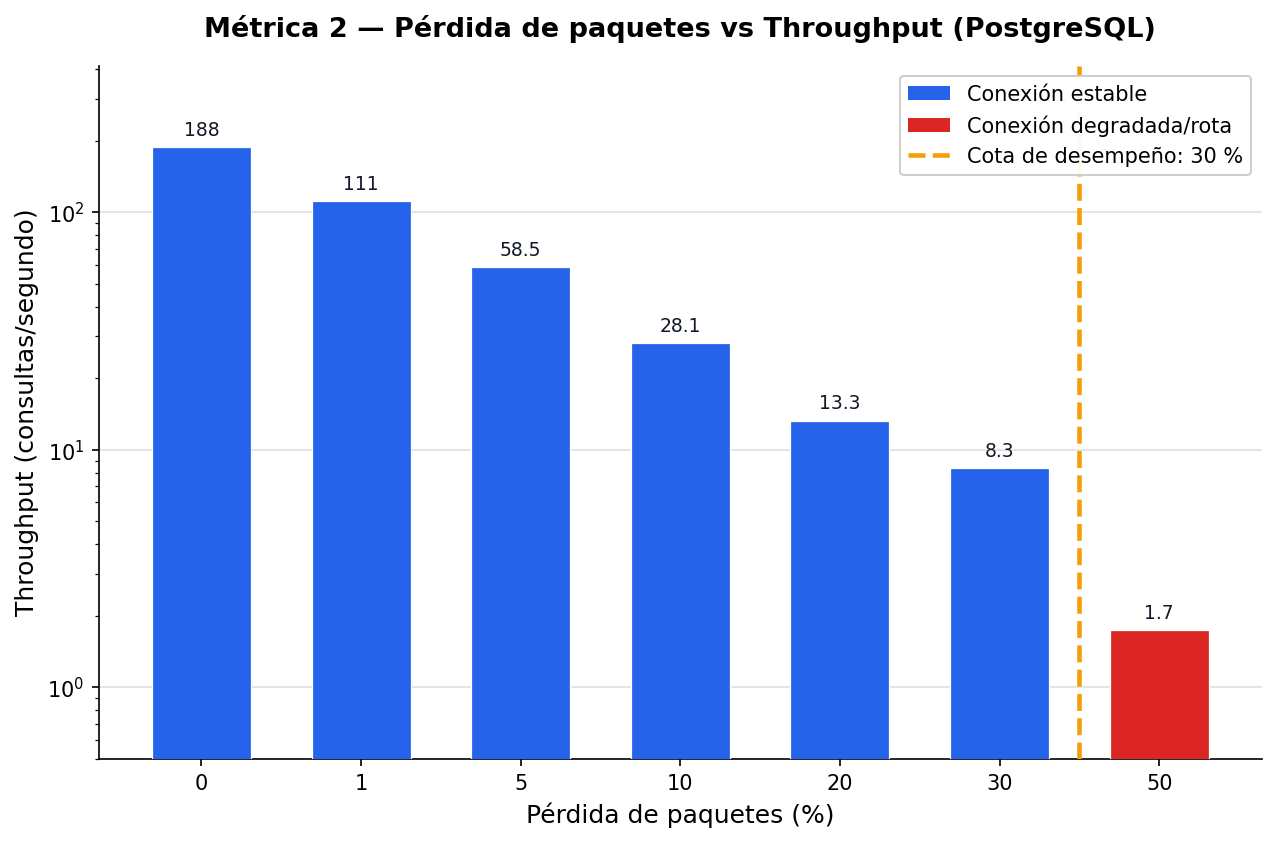
\includegraphics[width=\linewidth]{imagenes/grafico_perdida.png}
\caption{Métrica 2: pérdida de paquetes vs throughput. La línea punteada marca la
cota de desempeño.}
\end{figure}

\textbf{Cota de desempeño.} El servicio se mantiene utilizable hasta un
\textbf{30\,\%} de pérdida ($\approx$8{,}3~ops/s); a 50\,\% el throughput se
desploma a 1{,}7~ops/s ---menos del 1\,\% del valor base--- y las 100 consultas
tardan 57~s. La \textbf{cota de desempeño se sitúa en 30\,\%}. Un hallazgo
relevante de la medición real es que, gracias a las retransmisiones de TCP, la
conexión \emph{no se rompe} ni siquiera con un 50\,\% de pérdida: simplemente se
vuelve tan lenta que es inservible en la práctica. Como cada paquete perdido
cuesta un RTO completo, el throughput cae de forma mucho más abrupta que con la
latencia (de 188 a 1{,}7~ops/s).

% ===================== 7. CONCLUSIONES ==========================
\section{Conclusiones}

\textbf{Vulnerabilidades del protocolo sin TLS.} Las tres modificaciones
demuestran que, sin cifrado, el protocolo PostgreSQL es completamente
manipulable por un intermediario. El caso más grave es la Modificación~3: un
MITM puede reescribir la \emph{semántica} de las consultas ---inyectar latencia,
redirigir tablas o vaciar resultados--- sin que cliente ni servidor lo detecten,
porque el protocolo no integra verificación de integridad. Corromper el
encabezado (Modificaciones~1 y~2) no permite un ataque sigiloso, pero sí una
\textbf{denegación de servicio} trivial sobre la sesión.

\textbf{Robustez del servidor ante entradas malformadas.} Los dos experimentos
de \emph{fuzzing} y las modificaciones de encabezado confirmaron que el servidor
es \textbf{robusto}: validó tamaño, versión y estructura por capas, respondió con
errores \texttt{FATAL} controlados (\texttt{0A000}, \texttt{08P01}) o cerró la
conexión, pero el \emph{postmaster} nunca cayó. El aislamiento por proceso (un
\emph{fork} por sesión) contiene el daño a la sesión afectada.

\textbf{Cotas de desempeño.} Se identificaron cotas concretas para cada métrica:
\textbf{100~ms} de latencia y \textbf{30\,\%} de pérdida de paquetes. Ambas métricas miden
aspectos diferentes (retardo vs.\ fiabilidad) y degradan el throughput por
mecanismos distintos: la latencia lo hace de forma hiperbólica y predecible
($\sim 1/RTT$), mientras que la pérdida lo colapsa de forma abrupta por la
acumulación de retransmisiones.

\textbf{Importancia de TLS.} La conclusión transversal es que la confidencialidad
\emph{y} la integridad del servicio dependen por completo de habilitar TLS. La
misma posición de intermediario que permite el \emph{downgrade} descrito en la
Tarea~2 habilita todos los ataques de modificación de esta tarea. Configurar
\texttt{sslmode=require} (o superior) no es opcional en entornos reales: es la
única defensa contra la clase de ataques aquí demostrada.

% ===================== BIBLIOGRAFÍA ==========================
\begin{thebibliography}{99}
\bibitem{pgprotocol} The PostgreSQL Global Development Group.
  \emph{PostgreSQL 17 Documentation, Ch.~53: Frontend/Backend Protocol}, 2026.
  \url{https://www.postgresql.org/docs/17/protocol.html}
\bibitem{pgmessageformats} The PostgreSQL Global Development Group.
  \emph{PostgreSQL 17 Documentation, Sec.~53.7: Message Formats}, 2026.
  \url{https://www.postgresql.org/docs/17/protocol-message-formats.html}
\bibitem{pgsource} The PostgreSQL Global Development Group.
  \emph{PostgreSQL --- Repositorio oficial (GitHub)}.
  \url{https://github.com/postgres/postgres}
\bibitem{scapy} P. Biondi y la comunidad Scapy.
  \emph{Scapy --- Packet crafting for Python}. \url{https://scapy.net/}
\bibitem{netem} The Linux Foundation. \emph{netem --- Network Emulator,
  tc-netem(8)}. \url{https://man7.org/linux/man-pages/man8/tc-netem.8.html}
\bibitem{rfc5802} C. Newman, A. Menon-Sen, A. Melnikov, N. Williams.
  \emph{SCRAM SASL and GSS-API Mechanisms}, RFC 5802, IETF, 2010.
  \url{https://www.rfc-editor.org/rfc/rfc5802}
\bibitem{rfc9293} W. Eddy (ed.). \emph{Transmission Control Protocol (TCP)},
  RFC 9293, IETF, 2022. \url{https://www.rfc-editor.org/rfc/rfc9293}
\bibitem{mathis1997} M. Mathis, J. Semke, J. Mahdavi, T. Ott.
  \emph{The Macroscopic Behavior of the TCP Congestion Avoidance Algorithm}.
  ACM SIGCOMM CCR, 27(3):67--82, 1997.
\bibitem{takanen2008} A. Takanen, J. DeMott, C. Miller.
  \emph{Fuzzing for Software Security Testing and Quality Assurance}.
  Artech House, 2008.
\bibitem{dockernet} Docker Inc. \emph{Networking overview --- Docker
  Documentation}. \url{https://docs.docker.com/network/}
\end{thebibliography}

\end{document}
